% mnras_template.tex
%
% LaTeX template for creating an MNRAS paper
%
% v3.0 released 14 May 2015
% (version numbers match those of mnras.cls)
%
% Copyright (C) Royal Astronomical Society 2015
% Authors:
% Keith T. Smith (Royal Astronomical Society)

% Change log
%
% v3.0 May 2015
%    Renamed to match the new package name
%    Version number matches mnras.cls
%    A few minor tweaks to wording
% v1.0 September 2013
%    Beta testing only - never publicly released
%    First version: a simple (ish) template for creating an MNRAS paper

%%%%%%%%%%%%%%%%%%%%%%%%%%%%%%%%%%%%%%%%%%%%%%%%%%
% Basic setup. Most papers should leave these options alone.
\documentclass[a4paper,usenatbib]{mnras}
%BH: I commented out fleqn to make equations centered/prettier spaced

% MNRAS is set in Times font. If you don't have this installed (most LaTeX
% installations will be fine) or prefer the old Computer Modern fonts, comment
% out the following line
\usepackage{newtxtext,newtxmath}
% Depending on your LaTeX fonts installation, you might get better results with one of these:
%\usepackage{mathptmx}
%\usepackage{txfonts}

% Use vector fonts, so it zooms properly in on-screen viewing software
% Don't change these lines unless you know what you are doing
\usepackage[T1]{fontenc}
\usepackage{ae,aecompl}


%%%%% AUTHORS - PLACE YOUR OWN PACKAGES HERE %%%%%

% Only include extra packages if you really need them. Common packages are:
\usepackage{graphicx}	% Including figure files
\usepackage{amsmath}	% Advanced maths commands
\usepackage{amssymb}	% Extra maths symbols

%%%%%%%%%%%%%%%%%%%%%%%%%%%%%%%%%%%%%%%%%%%%%%%%%%

%%%%% AUTHORS - PLACE YOUR OWN COMMANDS HERE %%%%%

% Please keep new commands to a minimum, and use \newcommand not \def to avoid
% overwriting existing commands. Example:
%\newcommand{\pcm}{\,cm$^{-2}$}	% per cm-squared

\newcommand{\FL}[1]{{\color{magenta}FL: #1}}
\newcommand{\CH}[1]{{\color{green}CH: #1}}
\newcommand{\SF}[1]{{\color{cyan}SF: #1}}
\newcommand{\BH}[1]{{\color{red}BH: #1}}
\newcommand{\CM}[1]{{\color{cyan}CM: #1}}
% \definecolor{cmgray}{gray}{0.6}
\newcommand{\cmadd}[1]{{\color{green}#1}}
\newcommand{\dhod}{{\sc DiffHOD}}
%%%%%%%%%%%%%%%%%%%%%%%%%%%%%%%%%%%%%%%%%%%%%%%%%%

%%%%%%%%%%%%%%%%%%% TITLE PAGE %%%%%%%%%%%%%%%%%%%

% Title of the paper, and the short title which is used in the headers.
% Keep the title short and informative.
\title[DiffHOD]{Differentiable Stochastic Halo Occupation Distribution}

% The list of authors, and the short list which is used in the headers.
% If you need two or more lines of authors, add an extra line using \newauthor
\author[B. Horowitz et al.]{
Benjamin Horowitz,$^{1,2}$\thanks{E-mail: bhorowitz@princeton.edu}
ChangHoon Hahn,$^{1}$
Francois Lanusse,$^{3}$
Chirag Modi,$^{4,5}$ \newauthor Simone Ferraro$^{2}$
\\
% List of institutions
$^{1}$Department of Astrophysical Sciences, Princeton University, Princeton, NJ 08544, USA\\
$^{2}$Lawrence Berkeley National Lab, 1 Cyclotron Road, Berkeley, CA 94720, USA\\
$^{3}$AIM, CEA, CNRS, Universit\'e Paris-Saclay, Universit\'e Paris Diderot, Sorbonne Paris Cit\'e, F-91191 Gif-sur-Yvette, France\\
$^{4}$Center for Computational Astrophysics, Flatiron Institute, 162 Fifth Ave., New York, NY 10010, USA\\
$^{5}$Center for Computational Mathematics, Flatiron Institute, 162 Fifth Ave., New York, NY 10010, USA
}

% These dates will be filled out by the publisher
\date{Accepted XXX. Received YYY; in original form ZZZ}

% Enter the current year, for the copyright statements etc.
\pubyear{2020}

% Don't change these lines
\begin{document}
\label{firstpage}
\pagerange{\pageref{firstpage}--\pageref{lastpage}}
\maketitle

% Abstract of the paper
\begin{abstract}
In this work, we demonstrate how differentiable stochastic sampling techniques developed in the context of deep Reinforcement Learning can be used to perform efficient parameter inference over stochastic, simulation-based, forward models. As a particular example, we focus on the problem of estimating parameters of an Halo Occupancy Distribution (HOD) model. Using a combination of continuous relaxation and gradient re-parameterisation techniques, we can obtain well-defined gradients with respect to HOD parameters through discrete galaxy catalogs realisations. Having access to these gradients allows us to leverage efficient sampling schemes, such as Hamiltonian Monte-Carlo, and greatly speed up parameter inference.
%Using the Gumbel-Softmax approach, we can map the discrete HOD models to a continuous distribution with well defined derivatives, allowing the use of first order optimization methods, such as Hamiltonian Monte Carlo, for analysis of data.
We demonstrate our technique on a mock galaxy catalog generated from the Bolshoi simulation using the 
\cite{2007zheng} %Zheng et al. 2007 
HOD model and find %,finding 
comparable posteriors as standard Markov Chain Monte Carlo techniques approximately 20x faster. 
Our differentiable HOD model %This model 
also has broad applications in full forward model approaches to cosmic structure and cosmological analysis. 
\end{abstract}

% Select between one and six entries from the list of approved keywords.
% Don't make up new ones.
\begin{keywords}
methods: numerical -- cosmology: theory -- galaxies: haloes -- galaxies: fundamental parameters
\end{keywords}

%%%%%%%%%%%%%%%%%%%%%%%%%%%%%%%%%%%%%%%%%%%%%%%%%%

%%%%%%%%%%%%%%%%% BODY OF PAPER %%%%%%%%%%%%%%%%%%

\section{Introduction}

%plot comparing DiffHOD to HOD at PS level

%MCMC run with HOD parameters


Over the past twenty years, there as been significant observational and theoretical progress in connecting galaxies to their cosmic environments \citep{2000MNRAS.318.1144P,2003MNRAS.340..771V,kravtsov2004,2006ApJ...652...71W,2011MNRAS.414.1405N}. Understanding this connection is critical for understanding galaxy formation/evolution \citep{2009MNRAS.399.1773C,2011ApJ...736...59Z} as well as using galaxies as bias tracers of the underlying mass density for cosmological analyses \citep{2000MNRAS.311..793B,2018PhR...733....1D}. Studying this connection is a key component of a many upcoming galaxy surveys including the Prime Focus Spectrograph \citep{2016SPIE.9908E..1MT}, the Dark Energy Spectroscopic Instrument \citep{2016arXiv161100036D}, and the Nancy Grace Roman Space Telescope~\citep{2015arXiv150303757S}.

A key theoretical tool for these studies has been the Halo Occupation 
Distribution \citep[HOD;][]{lemson1999, benson2000, seljak2000, scoccimarro2001, 2002ApJ...575..587B, wechsler2018}, 
a framework that specifies how collapsed dark matter halos~\citep{press1974, bond1991, cooray2002} are populated with galaxies.
 %an abundance matching approach to map from dark matter halos to their constituent galaxies. 
This is in contrast to ``environmental" biasing schemes, such as Eulerian 
or Lagrangian biasing schemes \citep{1998MNRAS.293..209M, 2018PhR...733....1D}, 
common in 
%the analysis of galaxy survey data for cosmological analysis 
cosmological analyses of galaxy survey data \citep{2016MNRAS.457.1770C,2020JCAP...05..042I,2021PhRvL.126n1301T}.
Unlike environmental biasing schemes that %matches only models the summary statistics 
only model summary statistics
like power spectrum of the galaxy field,
a well-formulated HOD model provides direct physical insight into galaxy formation physics 
through its parameters, which are %as the parameters of an HOD 
related to critical mass scales in galaxy-halo relation. 
For example, this allows direct measurement of HOD parameters by comparing observed galaxy populations with dynamical mass measurements, such as x-ray clusters \citep{2009ApJ...707..554Z,2016MNRAS.463.1929M}. 
%\CH{fine --- but the physical meaningfulness of HOD is a bit overstated here}

In standard HOD implementations~\citep[\emph{e.g}][]{2005zheng},  %, such as that in the standard halotools implementation \citep{2016MNRAS.460.2552H}
the HOD model specifies the probability distribution of the number
of galaxies, $N$, hosted by a dark matter halo given its properties, such as halo 
mass: $P(N|M_{\rm halo})$. A semi-analytical halo-model approach can include HOD parameters to predict two and higher point function \citep{cooray2002}, but those predictions are often not accurate 
enough for analysing modern datasets. Alternatively, a more precise Monte Carlo approach is often used to stochastically assign galaxies to halos in a large simulation box following the HOD prescription, and then the galaxy power spectrum or other quantities of interest are directly measured from the simulation. 
% Formally this assignment is not differentiable as it is over a discrete categorical variable. 
% This greatly restricts the possible approaches for parameter fitting and error estimation. 

In practice, Markov-Chain Monte-Carlo methods have primarily been 
used to fit HOD parameters from mock or actual data~\citep[\emph{e.g.}][]{white2011, rodriguez-torres2016, sinha2018}. However these methods scale poorly with the number of parameters that need to be fit.
As novel decorated HOD models increasingly add more assembly bias parameters to accurately capture small scale observations,
this exercise can become challenging, especially if there are unforeseen degeneracies in the parameter space.
These challenges can be overcome more easily with parameter inference methods that rely on the gradient information 
\emph{i.e.} where we can estimate the response of the observations with respect to the underlying parameters of the model,
such as Hamiltonian Monte Carlo \citep{1987PhLB..195..216D} or Variational Inference \citep{peterson1987mean,2003PhDT.......250B,2016arXiv160100670B}.
However these methods are not applicable in current HOD models as the implementation of their stochastic galaxy assignment schemes make them classically non-differentiable. 

A differentiable HOD framework will enhance dynamical forward modelling frameworks that seek to reconstruct latent cosmological fields~\citep[\emph{e.g.}][]{2017JCAP...12..009S}
and are constrained to use gradient based methods for optimization due to the high dimensionality of the inference problem.
These frameworks generally rely on perturbative bias models that are accurate only on large scales \citep{Schmidt18, Modi19} 
or heuristic neural network models with a large number of latent parameters \citep{2018JCAP...10..028M}.
A differentiable HOD approach will allow one to push to smaller scales with a well-understood, physically developed model that has only a handful of parameters.
%\CH{we need a sentence or two on why we care about these gradient-based methods. perhaps provide some bigger picture context of DUI.} 

An alternative to HOD models that maintains the requisite differentiability is to use differentiable emulators \citep{2015ApJ...810...35K,2020MNRAS.492.2872W} or fitting functions of the observables like the one proposed in \citet{2021arXiv210505859H} for galaxy assembly bias. 
However these are efficient only for the particular summary statistics and cosmological parameters on which they are trained.
Hence, they require a new training set once these are varied. 
Depending on the parameter space of interest this could be of prohibitive computationally cost. 
In addition, separate emulators must be trained for each summary statistic of interest as such methods do not match the galaxy observations at the field level.

%\FL{Other emulators/fitting functions used for HMC that we can cite? We also want to say why they are annoying, like require a "training set" of simulations, not flexible, etc..}

Motivated by this, here we adopt a different approach and aim to make the HOD sampling itself differentiable.
Our aim is to be able to compute gradients of any observable with respect to HOD parameters through a particular realisation of a galaxy catalog. 
Common wisdom would states that differentiating through stochastically sampled discrete random variables, such as the number of satellites in a given halo, is not possible. 
However, modern Reinforcement Learning have spurred the development of techniques to deal with these types of categorical variables in the context of deep neural network training via back propagation. 
In particular, we use the Gumbel-Softmax or CONCRETE method \citep{2016arXiv161101144J,2016arXiv161100712M} 
that utilises continuous distributions to approximate the sampling process of discrete stochastic variables, such as galaxies, in a differentiable fashion. %\FL{this last sentence needs a little bit more work.}
It relies on two insights: 1) a re-parameterization for a discrete (or categorical) 
distribution in terms of the Gumbel distribution~\citep[referred to as the ``Gumbel trick''][]{2014arXiv1411.0030M} 
and 2) making the corresponding function continuous by using a continuous approximation that depends on a \textit{temperature} parameter, which in the zero-temperature case degenerates to the discontinuous, original expression. 


In this paper, we will implement the Gumbel - Softmax method in the context of HOD models and apply it to mock datasets. In Sec. \ref{sec:methods} we will describe our HOD model and the constructs used to allow differentiability of its categorical outputs. In Sec. \ref{sec:exp}, we apply this technique to a Monte Carlo analysis of a mock galaxy catalog constructed from the Planck-Bolshoi simulation. In Sec. \ref{sec:conclusion} we compare the differentiable HOD model to that from a standard approach and discuss its applications.

\section{Method}
\label{sec:methods}

In this section, we provide some background on the various components of our HOD model, and detail our strategy to make this model differentiable. We implement our model using Tensorflow Probability \citep{2016arXiv161009787T,morgan2018probabilistic}, particularly the Tensorflow Distribution package \citep{2017arXiv171110604D}. 

\subsection{HOD Model} \label{sec:hod}

To describe the population of galaxies in our halos we use the standard 
\cite{2007zheng} HOD model.
In the \cite{2007zheng} model, the probability of a given halo hosting 
$N$ galaxies is dictated solely by its mass --- $P(N|M)$.
The model separately populates central and satellite galaxies, motivated by
theoretical studies~\citep{kravtsov2004, 2005zheng}, and has five free parameters
with some physical significance that
can be related back to well studied mass-luminosity relationships.

\subsubsection{Central occupation}

For central galaxies, the mean occupation function is step-like with a soft cutoff to account for natural scatter between galaxy luminosity the halo host mass. There are two free parameters controlling this function, the characteristic minimum mass of halos hosting central galaxies above some luminosity threshold, $M_\textrm{min}$, and the width of the cutoff profile, $\sigma_{\log M}$:
\begin{equation}
    \langle N_\textrm{cen}(M) \rangle = \frac{1}{2} \left[ 1 + \textrm{erf}\left( \frac{\log M - \log M_\textrm{min}}{\sigma_{\log M}}\right)\right],
    \label{eq:ncen}
\end{equation}
where erf is the standard error function and $M$ is the halo mass. 
Given this value of the mean occupation for a halo of a given mass, the central is sampled using a Bernoulli distribution for each halo
\begin{equation}
    N_\textrm{cen} \sim \textrm{Bernoulli}\big( p = \langle N_\textrm{cen}(M) \rangle \big)
    \label{eq:ncensample}
\end{equation}
%\CH{explain how $N_{\rm cen}$ is sampled for each halo} 

\begin{figure}
    \centering
    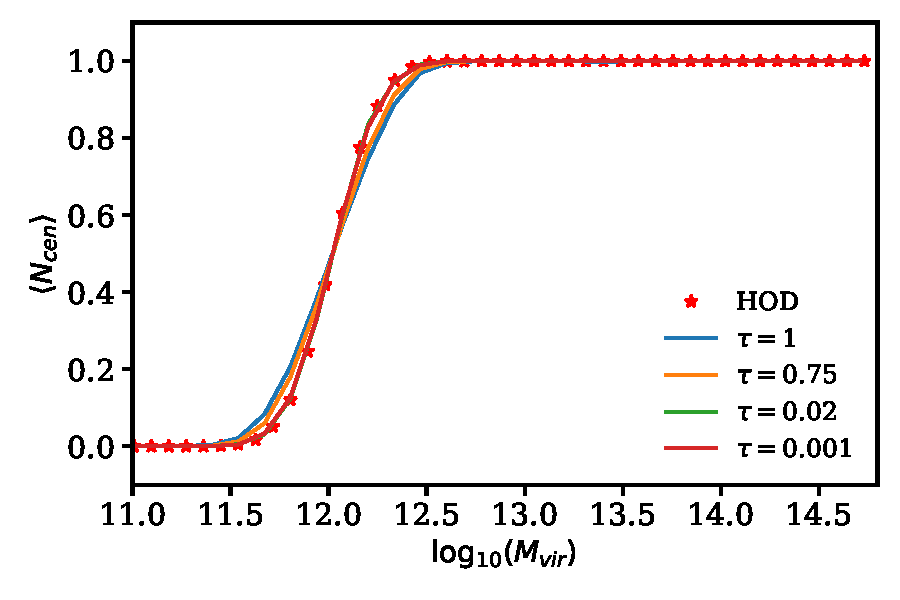
\includegraphics[width=0.45\textwidth]{paper/plots/occupancy_cen.pdf}
    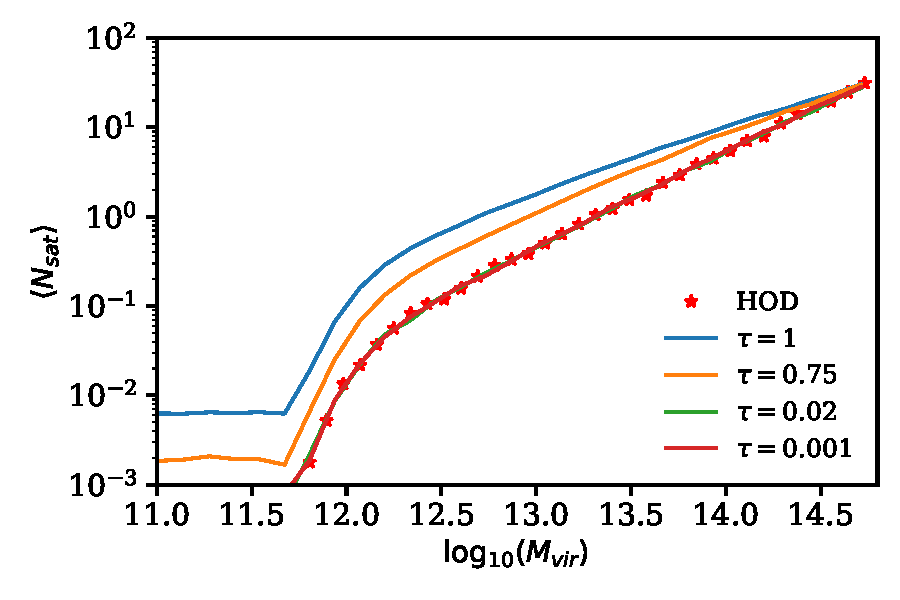
\includegraphics[width=0.45\textwidth]{paper/plots/occupancy_sat.pdf}
    \caption{\label{fig:occupancy}
    Halo occupancy distribution for central (top) and satellite galaxies (bottom) 
    as a function of halo virial mass of our differentiable HOD model (\dhod; solid).
    Different colors indicate different temperature values used in the Gumbel-Softmax 
    approximation (see Eq. \ref{eq:softmax}).
    We include the occupancy distribution from the standard \cite{2007zheng} HOD model for 
    reference (star). 
    In this work, we use \dhod~with $\tau=0.02$, which is in good agreement 
    with the standard HOD model throughout the full halo mass range.
    }
\end{figure}

\begin{figure*}
    \centering
    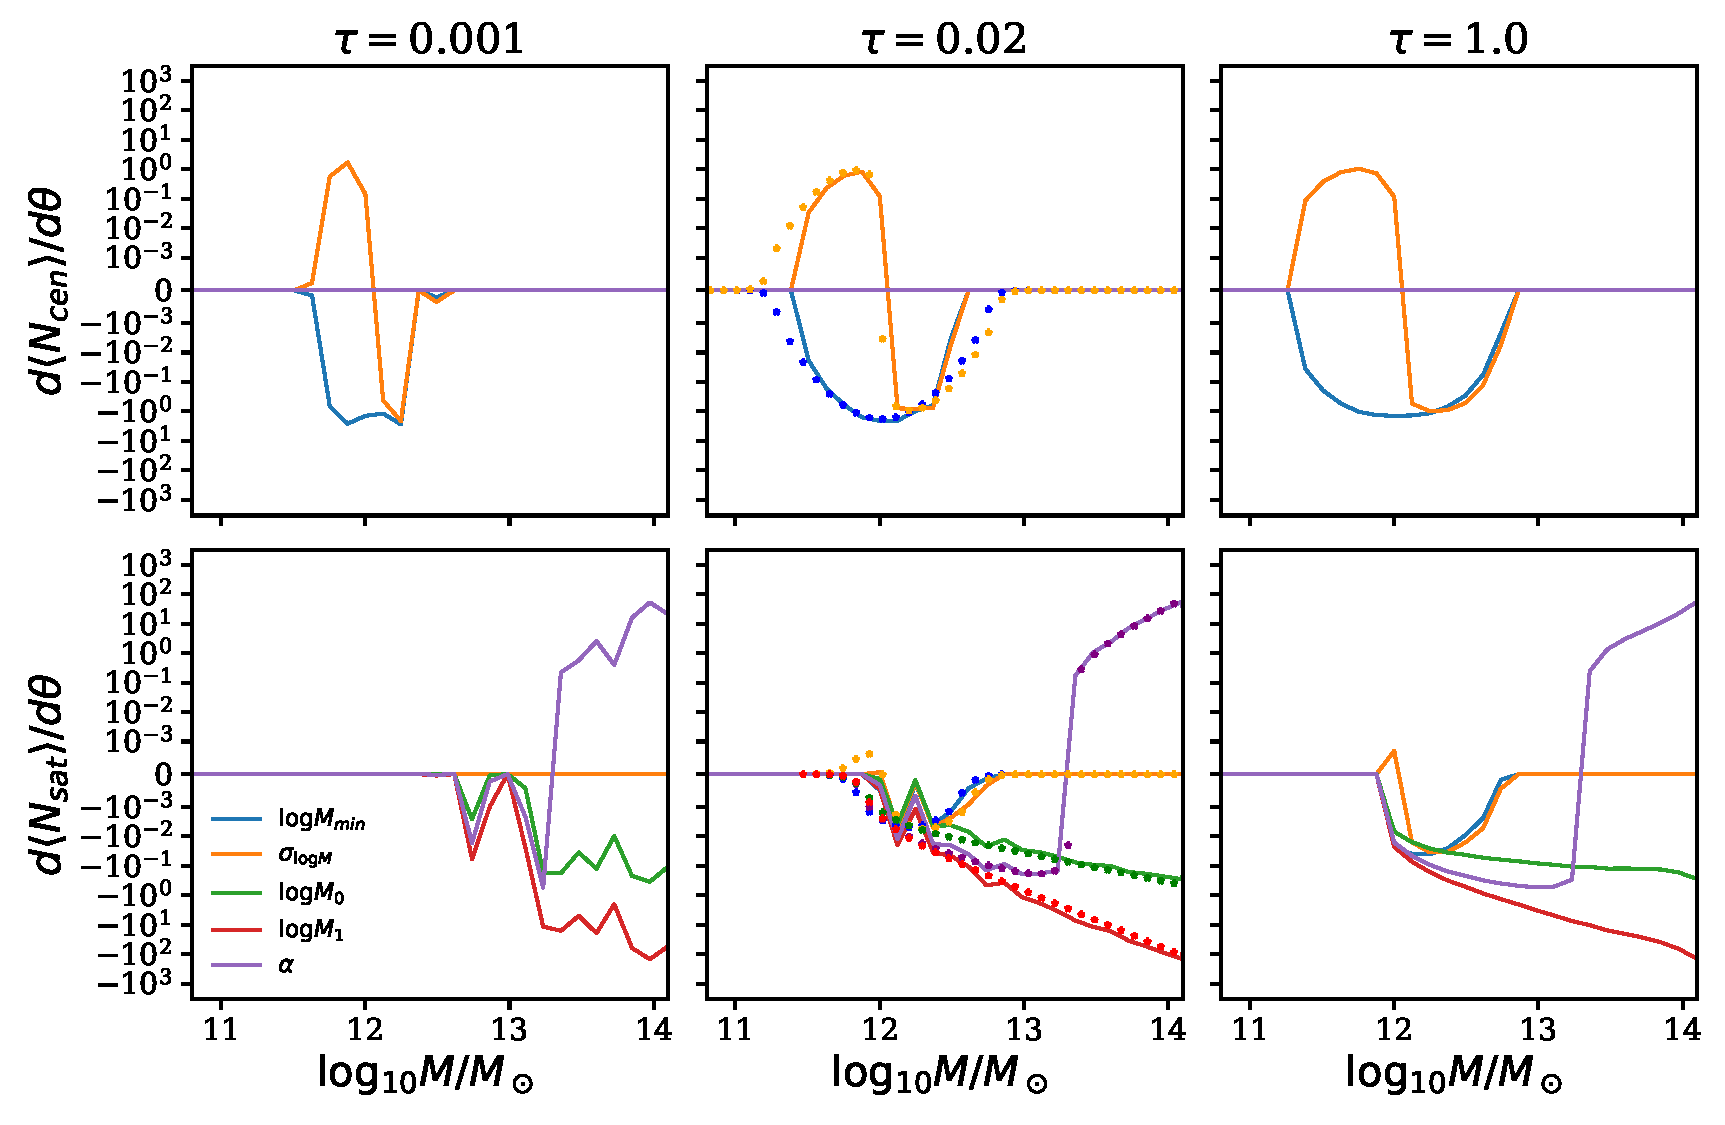
\includegraphics[width=0.70\textwidth]{paper/plots/3panel.pdf}
    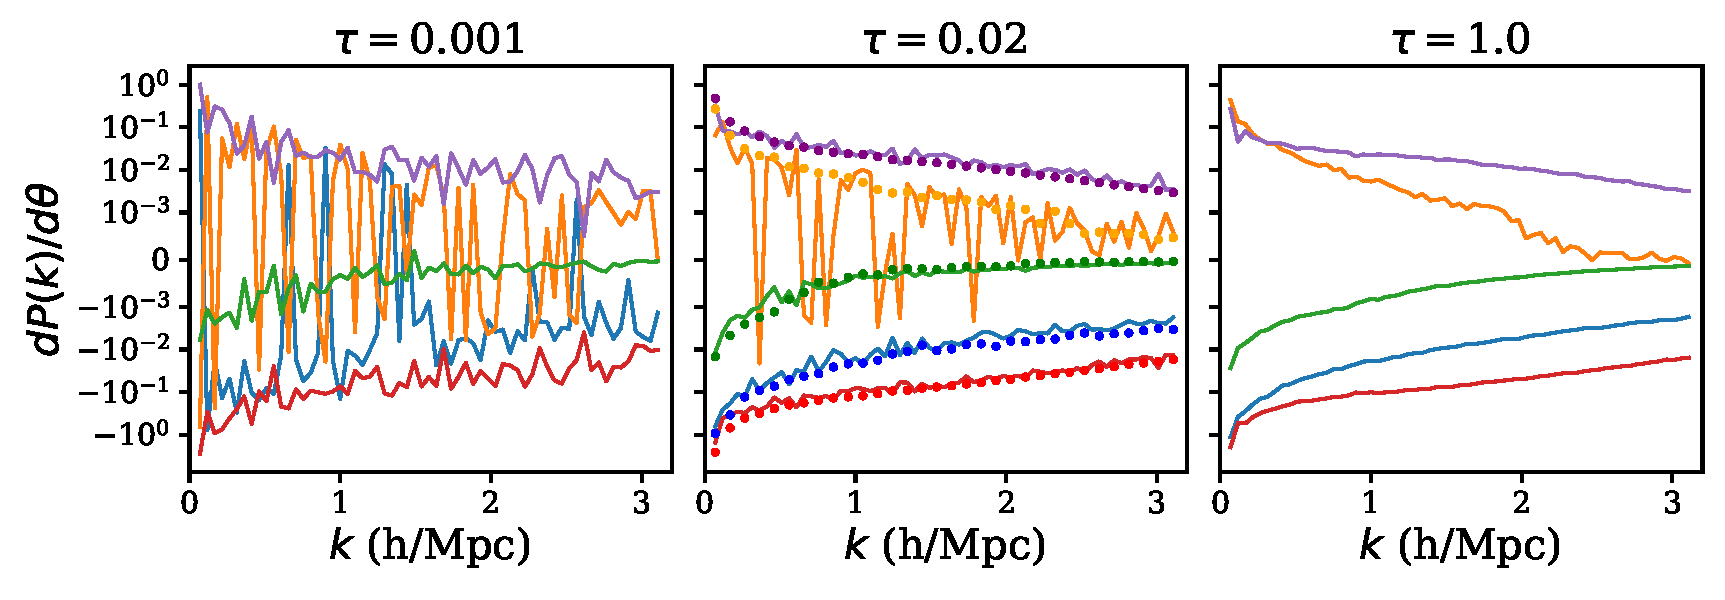
\includegraphics[width=0.71\textwidth]{paper/plots/ps_comparison.pdf}
    \caption{
    \emph{Top}: Derivatives of the central and satellite occupancy functions 
    with respect to the HOD parameters for various temperatures: $\tau=0.001$ 
    (left) 0.02 (center), and 1 (right). 
    The derivatives are calculated at the fiducial HOD parameter values. 
    We include derivatives analytically derived from Eqs.~\ref{eq:ncen} 
    and~\ref{eq:nsat} for comparison (star). 
    \emph{Bottom}: Derivatives of the galaxy power spectrum with respect to the 
    HOD parameters, evaluated at the fiducial HOD parameter values. 
    We include derivatives calculated using the standard HOD with finite 
    difference for comparison (star). 
    Our \dhod~model with $\tau=0.02$ provides sufficiently smooth derivatives that
    are in good agreement with analytical derivatives for the occupancy function 
    and with standard HOD derivatives for the power spectrum.
    %Small dots represent derives calculated analytically from Eq. \ref{eq:ncen} and Eq. \ref{eq:nsat} (top) and finite difference (bottom).
    \label{fig:occupancy_derivatives}}
\end{figure*}
\subsubsection{Satellite occupation}

Simulations suggest that satellites follow an approximately power-law distribution with a slope close to unity at the high mass end. At lower masses, the shape of the distribution changes and the overall distribution can be parameterized as
%\langle N_\textrm{sat}(M) \rangle = \frac{1}{2} \left[ 1 + \textrm{erf}\left( \frac{\log M - \log M_\textrm{min}}{\sigma_{\log M}}\right)\right]\left( \frac{M-M_0}{M_1'}, \right)^\alpha,
\begin{equation}
    \langle N_\textrm{sat}(M) \rangle = \langle N_{\rm cen}(M) \rangle \left( \frac{M-M_0}{M_1'} \right)^\alpha,
    \label{eq:nsat}
\end{equation}
where $\alpha$ is the power law slope at high masses, $M_0$ is the characteristic mass of the change-over and $M_1'$ is the characteristic amplitude.  This mean number of satellites for a given mass is then used to define the intensity $\lambda$ of a Poisson distribution, from which a particular number of satellites are drawn for each halo.
\begin{equation}
    N_\textrm{sat} \sim \textrm{Poisson}\big(\lambda = \langle N_\textrm{sat}(M) \rangle \big)
    \label{eq:nsatsample}
\end{equation}
%hodpy \cite{2017MNRAS.470.4646S}, 

%\CM{Do we worry about the fact that some models do not have satellites in the halos that do not have any centrals?}

\subsubsection{Spatial satellite distribution}

In the \cite{2007zheng} HOD, central galaxies are located at the center 
of its host halo and satellite galaxies are distributed according to a 
\cite{nfw1997} profile (hereafter NFW).
To sample the satellite galaxy positions, we utilize the \cite{2018RNAAS...2...55R} 
implementation, which constructs an efficient mapping from a random sample 
and the full NFW profile via the calculation of the quantile function, 
\emph{i.e.} the inverse Cumulative Distribution Function (CDF). 
This can be written analytically as
\begin{equation}
    q(p;c) = -\frac{1}{c}\left[ 1 + \frac{1}{W_0(-e^{-pM_{\rm vir}-1})} \right],
    \label{eq:NFW}
\end{equation}
where $W_0$ is the Lambert-W function, $M_{\rm vir}$ is the virial mass and $c$ is the concentration parameter. Using this inverse CDF, we can now randomly draw radial distances for satellites by sampling  $p$ from $U[0,1]$ and mapping it to radii as $r/r_{\rm vir} = q(p,c)$. The angular position of the satellite is sampled uniformly in this isotropic model.%We can generate samples following the NFW profile now by sampling $p$ from $U[0,1]$.
%\CH{more details needed on how this actually translates to satellite position.}

\subsection{Differentiable stochastic sampling}

In this section, we review the key ideas behind differentiable stochastic sampling, which will form the building blocks of DiffHOD.

\subsubsection{Stochastic backpropagation by reparametrisation}

One of the most common approaches for backpropagation through stochastic sampling is the so-called reparametrisation trick, extensively used for instance in Variational Auto-Encoders \citep{Kingma2013,Rezende2014}. 

The key idea of this approach is to rewrite samples $z$ from a given paramteric distribution $\mathbb{P}_{\theta}$ as a deterministic and differentiable transformation $f$ applied to a fixed distribution $\mathbb{P}_{\epsilon}$:
\begin{equation}
    z = f(\theta, \epsilon) \mbox{ with } \epsilon \sim \mathbb{P}_{\epsilon} 
\end{equation}
This reparametrisation of the samples allows to side-step having to take derivatives of the stochastic variable $\epsilon$ when computing derivatives of some downstream function $h$ with respect to the distribution parameters $\theta$:
\begin{equation}
    \frac{\partial}{\partial \theta} \mathbb{E}_{z \sim p_\theta}\left[ h(z) \right] = 
    \mathbb{E}_{\epsilon \sim p_\epsilon} \left[ \frac{\partial}{\partial \theta} h(f(\theta, \epsilon)) \right] %= \mathbb{E}_{\epsilon \sim p_\epsilon} \left[ \frac{\partial h}{\partial f}  \frac{\partial f}{\partial \theta} \right]
\end{equation}
In the right-hand side of this expression, the derivative now only involves taking gradients of a deterministic function of $\theta$. 

To provide a simple concrete example of such reparameterisation, let us consider a Gaussian distribution of mean $\mu$ and standard deviation $\sigma$. One can express a sample $z \sim \mathcal{N}(\mu, \sigma^2)$ as $z = \mu + \sigma \epsilon$ with $\epsilon \sim \mathcal{N}(0, I)$, making it trivial to take derivatives of the samples with respect to the parameters of the distribution ($\mu$ and $\sigma$).

\subsubsection{Gumbel-Softmax trick for categorical variables}

The reparameterisation trick as presented above requires the samples to be expressible as a deterministic and differentiable function of a random variable. While this can often be achieved for continuous distributions, it is typically not directly possible for discrete categorical variables. 
To overcome this limitation, the Gumbel-Softmax trick \citep{2016arXiv161101144J,2016arXiv161100712M} introduces a relaxation of a categorical distribution to a continuous distribution, which can then be handled with the reparameterisation trick.

%We review here the Gumbel-Softmax trick as developed in the literature \citep{2016arXiv161101144J,2016arXiv161100712M} to map from categorical variables to a continuous differentiable distribution. 
Let $z$ be a categorical variable with class probabilities $\pi_1,\pi_2,...\pi_j$ that we wish to sample.
We assume that categorical samples are encoded as $j$-dimensional one-hot vectors, 
\emph{i.e.} they are 1$\times j$ vectors with all elements 0 except the
the element corresponding  to the sampled class which is 1. 
The simplest way to sample z is by 
\begin{equation}
    z = \textrm{onehot}(\textrm{max}{\, i | \pi_1 + ... + \pi_{i-1}\leq U}), \quad U \sim \textrm{Uniform}(0, 1)
    \label{eq:naivesampling}
\end{equation} 
A first step towards making these samples differentiable is to use the Gumbel-Max trick \citep{gumbel1954statistical,2014arXiv1411.0030M}, which reparametrizes categorical sampling as 
\begin{equation}
    z = \textrm{onehot}\left(\textrm{argmax}_{i}[g_i + \log{(\pi_i)}]\right),
    \label{eq:reparametrize}
\end{equation}
where $g_i$ are i.i.d. random variables drawn from the Gumbel distribution between 0 and 1, $\textrm{Gumbel}(0, 1)$\footnote{The standard Gumbel distribution is defined by cumulative distribution function $\textrm{CDF}(x) = \exp(-\exp(x))$ and probability density function, $\textrm{PDF}(x) = \exp(-(x+\exp(-x))$.}. 
This reparameterization trick refactors the sampling of $z$ into a deterministic function of the parameters ($\pi$) and some independent noise with a fixed distribution.
%As a result, now gradients are propagated w.r.t. parameters of a deterministic function instead of computing the gradient w.r.t. parameters of a distribution in Eq. \ref{eq:naivesampling}, which is a harder problem.

However the reparametrized function is still non-differentiable due to the $\textrm{argmax}$ function.
A continuous, differentiable approximation to this is given by a softmax function, 
\begin{equation}
    \mathrm{softmax}(\mathbf{z}, \tau )_i = \frac{\mathrm{e}^{z_i/\tau}}{\sum_{j=1}^k \mathrm{e}^{z_j/\tau}}, \quad \mathbf{z} = (z_1, z_2,...,z_k)
 \end{equation}
where $\tau$ is a free parameter sometimes referred to as the ``temperature".

Using this approximation relaxes the discreteness of the Gumbel-Max trick and generates a $k$-dimensional vector $\mathbf{z}$ 
\begin{equation}
    \hat{z}_i = \frac{\exp((\log(\pi_i)+g_i)/\tau)}{\sum_j \exp((\log(\pi_j)+g_j)/\tau)},
    \label{eq:softmax}
\end{equation}
We recover the true discrete function in the limit of $\tau \rightarrow 0$.
As this function is analytical in class probabilities $\pi$ for $\tau > 0$,
we can estimate the gradients of the observed samples $\mathbf{z}$ with respect to the parameters parameterizing $\pi$.

In practice, as $\tau$ approaches 0, gradients of our model mayb become unstable due to sensitivity to numerical precision. We explore the impact of this parameter in Sec.~\ref{sec:exp}.

\subsection{DiffHOD implementation} \label{sec:dhod}

We now have all the elements needed to build DiffHOD as a differentiable version of the HOD presented in Sec.~\ref{sec:hod}. We describe in this section our strategy for sampling central and satellites occupation, and satellites positions.

\subsubsection{Differentiable central occupation sampling}

As described in Sec.~\ref{sec:hod}, the central occupation is defined by a Bernoulli distribution, with a parameter $p=\left\langle N_{cen}(M | M_\mathrm{min}, \sigma_{\log M})\right\rangle$ defined as a deterministic function. 

Here, we can directly apply the Gumbel-Softmax trick introduced above thanks to the fact that the categorical distribution reduces to a Bernoulli distribution for when the number of classes is equal to 2. We therefore sample the central occupation for each halo as:
\begin{equation}
 N_{cen} = \frac{\exp((\log(p)+g_0)/\tau)}{\exp((\log(p)+g_0)/\tau) + \exp((\log(1-p)+g_1)/\tau) }\;.   
\end{equation}
with $g_1,g_0 \sim \textrm{Gumbel}(0, 1)$.
\FL{Check that this is actually what we do.... looks like TFP is using a different formula for the binary case, BinConcrete variable from Madison 2016.}


\subsubsection{Differentiable satellite occupation sampling}

For satellites, we aim to define a differentiable approach to sampling from a Poisson distribution with intensity $\lambda=\left\langle N_{sat}(M | M_0, M_1^\prime, \alpha)\right\rangle$, also a deterministic and differentiable function.

To build on the Gumbel-Softmax trick, we propose to replace conventional Poisson sampling of the total number of satellites by sampling the satellites from a Binomial distribution. We consider that every halo can have a maximum of $j$ satellites, then for each potential satellite, we define a Bernoulli distribution describing whether this satellite will be included for that particular halo. \FL{explain how this corresponds to Binomial, write the actual equation used for sampling}

While the resulting distribution is not strictly Poisonnian \FL{if it's not Poisson, how is it different exactly?}, it does verify the same mean number of galaxies. The variance of the distributions may be slightly skewed (see Appendix \ref{ap:1}), but we show that this does not result in appreciable biases of summary statistics or inferred parameters. \FL{Interestingly, Binomial tends to Poisson for n -> infty and n*p fixed, so we can say this is an approximation of the Poisson distribution. Also known as the law of rare events. Apparently a common rule of thumb is n > 100 and n*p < 10}

As a practical consideration, this procedure assumes a maximum number $j$ of satellites, i.e. a maximum number of Bernoulli draws. This is required for expressing the sampling as a function of arrays of fixed sizes. A higher value of $j$ can improve accuracy but it also increases memory costs, which scales linearly with the maximum number of satellite galaxies 
encoded in our one-hot embedding.
Meanwhile, too low of a $j$ can bias results by artificially truncating 
the satellite galaxies of the most massive halos. 

Our fiducial choice in this work is $j = 30$. In Fig.~\ref{fig:occupancy} (bottom), we can see that the satellite population reaches a maximum of $\sim 30$ galaxies for the most massive $\sim 10^{15} M_\odot$ halos. For the mass range considered here, we find $j > 30$ does not significantly improve the statistical match in summary statistics (correlation function, power spectra, etc.) of the resulting galaxy fields.
If the end statistic of interest is particularly sensitive to galaxy populations in the most massive clusters, a higher $j$ might be needed. If one is limited by memory or implementing HOD for halos with a broader mass range, then it may be more efficient to have multiple
halo mass bins with different maximum number of allowed satellites $j$.

\FL{WIP: still writing this section}

% We consider that every halo can have at-most one central and maximum of $j$ satellites. 
% Then for every galaxy, we define a categorical distribution with two classes, \textit{in=1} and \textit{out=0}
% where class \textit{in} corresponds to the galaxy being included for that particular halo. 
% The sampling probabilities $\pi_{\mathrm{in}}$ for centrals and satellites are  given by Eq. \ref{eq:ncensample} and \ref{eq:nsatsample} respectively. 
% We then use the Gumbel-Softmax trick as described in the previous section to sample $z$ for every galaxy between these two classes.
% The number of galaxies sampled in class $1$ corresponds to the total number of satellite galaxies. 
% The sampling of the satellite galaxy locations from the NFW is directly differentiable since it is a continuous variable which can be sampled directly from a uniform distribution, see Eq. \ref{eq:NFW}. 

% It is worth noting that such sampling corresponds to a relaxed Bernoulli distribution
% which is the correct distribution for the centrals, but not the satellites.
% However using the satellite Poisson parameter $\lambda$ for the Bernoulli distribution
% still results in the correct mean number of galaxies. Variance of the distributions may be slightly skewed (see Appendix \ref{ap:1}), but we show that this does not result in appreciable biases of summary statistics or inferred parameters. 

\subsubsection{Differentiable sampling from NFW distribution}

\FL{Write down exactly how we make the position of satellites differentiable, in terms of a mask + reparam of NFW distribution.... hum... even if we don't need to take gradients of NFW here...}.

%For HOD model, we are interested in sampling the number of centrals and satellites in a given halo. 

\subsubsection{Impact of temperature parameter $\tau$}

Temperature, $\tau$, is a free parameter in our model.
Depending on the context/implementation, it may be beneficial to anneal (i.e. reduce) $\tau$ over the course of the optimization such that $\tau \rightarrow 0$. For instance, in the original papers \citep{2016arXiv161101144J,2016arXiv161100712M}, the Gumbel-Softmax trick was used in the context of training a neural network where only the optimal network weights were of interest and hence $\tau$ was reduced to nearly zero over the course of the training.
However in our case, we are interested in stochastic sampling, and not 
optimization, so we will pick a single temperature that well approximates 
the target distribution (i.e. unbiased) while maintaining reasonable 
derivative properties (i.e. less noisy). 

%We show in Figure \ref{fig:occupancy} how the occupancy distributions change as a function of temperature compared to the that sampled from halotools.
In Fig.~\ref{fig:occupancy}, we present the central (top) and 
satellite (bottom) occupancy distributions of our differential HOD 
model (hereafter \dhod) for different temperatures: 
$\tau = 0.001$ (red) 0.02 (green), 0.75 (orange), and 1 (blue). 
We include the occupancy distributions for the standard HOD model for
comparison (star).

For this work, we find that a fixed $\tau=0.02$ provides high accuracy 
while maintaining stable gradients for both sampling the number of 
galaxies in each halo as well as the positions of the satellites from 
the NFW profile (see later Fig.~\ref{fig:occupancy_derivatives}). 
This experimental approach for determining $\tau$ was advocated for in \citet{2016arXiv161100712M}:
the temperature should set as high as possible while maintaining the 
desired accuracy of the target distribution. 

%There is an additional trade-off for the maximum dimension of the one-hot embedding, $j$. Memory costs scale linearly with maximum number of satellite galaxies encoded in our one-hot embedding, $j$, but setting too low of a $j$ can result in biases due to artificially truncating the satellite galaxies of the most massive halos. 
%In Figure \ref{fig:occupancy} (bottom), we can see the satellite population reaching a maximum of $\sim 30$ galaxies for the most massive $\sim 10^{15} M_\odot$ halos and so we choose $j=30$. 

% For the maximum dimension of the one-hot embedding, we use $j = 30$, 
% based on the occupation distributions.
% In Fig.~\ref{fig:occupancy} (bottom), we can see that the satellite 
% population reaches a maximum of $\sim 30$ galaxies for the most massive 
% $\sim 10^{15} M_\odot$ halos.
% A higher value of $j$ can improve accuracy but it also increases memory 
% costs, which scales linearly with the maximum number of satellite galaxies 
% encoded in our one-hot embedding.
% Meanwhile, too low of a $j$ can bias result by artificially truncating 
% the satellite galaxies of the most massive halos. 

% For the mass range considered here, we find $j > 30$ does not significantly improve the statistical match in summary statistics (correlation function, power spectra, etc.) of the resulting galaxy fields.
% If the end statistic of interest is particularly sensitive to galaxy populations in the most massive clusters, a higher $j$ might be needed. If one is limited by memory or implementing HOD for halos with a 
% broader mass range, then it may be more efficient to have multiple
% halo mass bins with different maximum number of allowed satellites $j$.


% \subsection{Differentiable Implementation}

% In order to perform derivative based optimization we need to transform the non-differentiable stochastic assigning of galaxies to a differentiable counterpart. To do so we will use the Gumbel-Softmax technique \cite{2016arXiv161101144J,2016arXiv161100712M} \FL{This should be Madison 2014, but I guess Jang et al 2016 is enough}, a reparametrization technique to map from categorical variables to a continuous differentiable distribution. 

% Let $z$ be the number of galaxies in a given halo, with associated probabilities $(\pi_1, \pi_2, \cdots, \pi_j)$, for some maximum number of galaxies $j$. For each halo, we will treat its galaxy population as a one-hot vector embedding in a $j$-dimensional space, treating separately the satellite and central populations. For centrals we have $j=1$. We can draw samples from this distribution via the following function;
% %\CM{Should say that this is done independently for centrals and satellites? Or not?}
% \begin{equation}
%     z = \textrm{onehot}\left(\textrm{argmax}(g_i + \log{(\pi_i))}\right),
% \end{equation}
% where $g_i$ are random variables drawn from the Gumbel distribution between zero and 1. The argmax function can be made differentiable with the softmax function to make our overall approximate function
% \begin{equation}
%     \hat{z}_i = \frac{\exp((\log(\pi_i)+g_i)/\tau)}{\sum_j \exp((\log(\pi_j)+g_j)/\tau)},
%     \label{eq:softmax}
% \end{equation}
% where we recover the true discrete function in the limit of $\tau \rightarrow 0$, where $\tau$ is sometimes referred to as the ``temperature." As this function is analytical in $\pi$ for $\tau > 0$, we can perform standard back-propagation through our model during optimization. In practice, as $\tau$ approaches 0, gradients of our model become unstable due to sensitivity to numerical precision. 

% Depending on the context/implementation, it may be beneficial to anneal (i.e. reduce) $\tau$ over the course of the optimization. In the original papers \citep{2016arXiv161101144J,2016arXiv161100712M}, the Gumbel Softmax trick was used in the context of training a neural network where only the optimal network weights were of interest. In \citet{2016arXiv161101144J}, $\tau$ was reduced to nearly zero over the course of the training, however in our case we are interested in stochastic sampling so we will pick a single temperature that both well approximates the target distribution while maintaining reasonable derivative properties. 

% We show in Fig \ref{fig:occupancy} how the occupancy distributions change as a function of temperature compared to the that sampled from halotools. For this work, we find that a fixed $\tau=0.02$ provides high accuracy while still maintaining stable gradients for both sampling the number of galaxies in each halo as well as the the positions of the satellites from the NFW profile. This experimental approach for determining $\tau$ was advocated for in \citet{2016arXiv161100712M}; $\tau$ should set as high as possible while still maintaining the desired accuracy of the target distribution. 

% There is an additional trade-off for the maximum dimension of the one-hot embedding, $j$. Memory costs scale linearly with maximum number of satellite galaxies encoded in our one-hot embedding, $j$, but setting too low of a $j$ can result in biases due to artificially truncating the satellite galaxies of the most massive halos. In Figure \ref{fig:occupancy} (bottom), we can see the satellite population reaching a maximum of $\sim 30$ galaxies for the most massive $\sim 10^{15} M_\odot$ halos and so we choose $j=30$. We find setting a higher $j$ does not significantly improve the statistical match in any summary statistics (correlation function, power spectra, etc.) of the resulting galaxy fields. If the end statistic of interest is particularly sensitive to galaxy populations in the most massive clusters,  a higher $j$ might be needed. For memory reasons, one can separate out the most massive halos into a separate class with a higher $j$.

    %\CH{We should get rid of $\tau=.0001$ panels, which I think will be more confusing than anything. 
    %How come the Nsat derivatives in the top panel go to 0 at 14 for DiffHOD while it continues for the HOD?  
    %We also need to have consistent x label as Figure 1. Hm, why is the DiffHOD so much noisier than finite differences? }\BH{I think a low temperature example is nice to show why $\tau = 0.02$ was choosen, but maybe $\tau=.0001$ is too low. I don't know why it goes to zero about $10^{14}$, I was playing around with it a lot and couldn't find a reason. WRT why DiffHOD is noisier, I attribute it to the numerical nature of the relaxed distribution we are using. At the high temperature limit we get a similarly smooth distribution.} 
    
%\SF{$10^{15} M_\odot$ halos and above can have way more than 30 satellites. Could this be related to the large-scale PS deviation that we see in Fig 3? But that will only affect large scales.} 

%\FL{
%Checks and plots that we might want to see here:
%  - Plot of smoothed distribution at different temperature
 % - Checking the power spectrum as a function of temperature
%  - Checking the gradients as a function of temperature
%  - Additional figures showing the HOD number density as function of temp
%}

\section{Experimentation}
\label{sec:exp}

%\CH{I think we should switch many of the references to halotool tools to just ``the standard''. 
%Halotools isn't some seminal package in the field so I think this will be confusing to people.}\BH{Happy to change the nomenclature! It might be nice to have a paragraph summarizing the different implementations and why we choose to use halotools for our comparison.}

To test our implementation, we construct a mock galaxy catalog from the Planck Bolshoi simulation halo catalog
\citep{2011Bolshoi} at $z=0$. This simulation has a  side length of 250 $h^{-1}$ Mpc, and contains 1367493 unique halos ranging in mass from $1.1 \times 10^{15} M_\odot$ down to $2.7 \times 10^{8} M_\odot$. We use halotools \citep{2016MNRAS.460.2552H} to generate our fiducial catalog with 
\cite{2007zheng} HOD parameter values: 
\begin{gather*}
    \log{M_\textrm{min}}=12.02,  \sigma_{\log{M}}=0.26, \log M_0 = 11.38, \\  \log{M_1}=13.31, \alpha = 1.0.
\end{gather*}
We construct a parallel galaxy catalog using our differentiable HOD implementation as described in Sec. \ref{sec:methods}. The galaxy catalogs are then painted onto a grid using a differentiable Cloud-In-Cell (CIC) painting method \citep{2020arXiv201011847M} and its power-spectra calculated via a differentiable Tensorflow power spectrum implementation \citep{2021TARDISII}.
%\CH{You've probably checked this but did you compare whether you get the discrepancy 
%in Figure 3 if you calculate the power spectrum with nbodykit rather than the 
%differentiable CIC and power spectrum? If so, I think that should be mentioned 
%somewhere.} \BH{Yeah, I checked the nbody PS implementation vs my PS implementation and the differences are very small $<0.1\%$.}

For \dhod, all steps are differentiable so the overall mapping from 
original halo catalog to end power spectrum is also differentiable via the
chain rule. 
%\CH{why cumulative?} 
In Fig.~\ref{fig:occupancy_derivatives}, we present the \dhod~derivatives 
of the central and satellite occupancy distribution functions (top)
and resulting power spectra (bottom) with respect to the HOD parameters
for different temperatures: $\tau = 0.001$ (left), $0.02$ (middle), and $1$ (right). 
The derivatives are evaluated at the fiducial HOD parameter values. 
With $\tau=0.001$, the power spectrum derivatives are dominated by numerical noise. 
The $\tau = 1.0$ derivatives are smoother but we find inaccurate occupancy
distributions (Fig.~\ref{fig:occupancy}) and a significantly biased power 
spectrum.
Meanwhile, with $\tau = 0.02$ there is still some noticeable numerical noise
in the derivatives, however, this is sufficiently smooth for our application 
and for our optimization to be well behaved. 
We also find that the $\tau=0.02$ \dhod~derivatives are in good agreement with
analytical derivatives for the occupancy function and with standard HOD derivatives 
estimated using finite differences for the power spectrum.

%We find the derivatives from this process match well those found via analytical calculation of the HOD model or those from finite differences of the resulting power spectrum. 
%\FL{Did I miss it or are we not mentioning anywhere that we are actually with non perfect derivatives because of the metropolis hastings step in the HMC?}
%\CM{Not sure what you mean}

We compare the differentiable power spectrum from our \dhod~model to the power 
spectrum from the standard HOD model in Figure~\ref{fig:ps}.
We use the fiducial HOD parameter values and estimate the error bars from 500 
realizations of our \dhod~model. 
We find good agreement (better than $3\%$) across all scales, with particularly
good agreement for central galaxies, which are not sampled from the NFW profile. Low $k$ modes are most sensitive to the most massive halos whose satellite 
galaxy populations may be truncated by our one-hot distribution 
($j=30$; Section~\ref{sec:dhod}).
However, even at $k < 0.15 h/{\rm Mpc}$, we find good agreement between the power spectra.
    
\begin{figure}
    \centering
    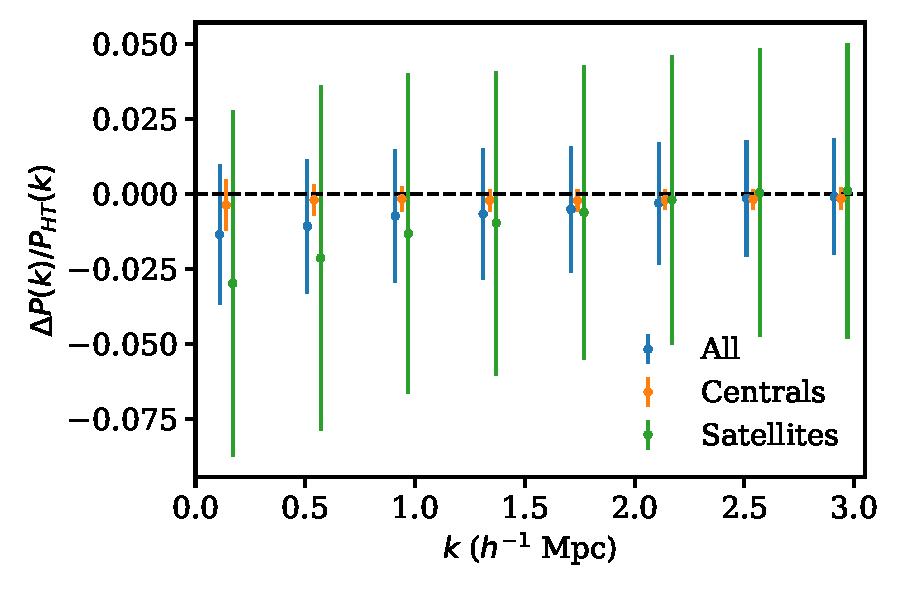
\includegraphics[width=0.50\textwidth]{paper/plots/ps_error.pdf}
    \caption{
    Comparison of power spectrum derived using a standard HOD model ($P_{\rm std}$)
    versus our \dhod~model. 
    We plot the ratios for central and satellite galaxies, as well as for all galaxies. 
    Error bars represent the standard deviation of the \dhod~model estimated from 
    500 realizations of the galaxy sampling.
    We find good agreement between the differentiable power spectrum and $P_{\rm std}$ 
    across all scales ($k < 3 h/{\rm Mpc}$).
    }
    \label{fig:ps}
\end{figure}

We now want to find the posterior on HOD parameters based on the observed power-spectra of the mock galaxy catalogs. We optimize for the HOD parameters within our differentiable forward model.
For demonstration, we use the same halo catalog as used to construct the mock catalog so the only source of error is variation caused by the HOD model. We construct a covariance matrix for our power spectra around a fiducial HOD parameter set for use in our likelihood calculation.

We perform a Hamiltonian Monte Carlo analysis of our model, sampling over the HOD parameters, using three chains initialized around our fiducial HOD parameters over 5,000 steps (with 300 steps of burn-in). This takes approximately 5 hours on a single Tesla V100-PCIE-32Gb GPU. For comparison, we run the same analysis using the standard HOD. 
Since this implementation does not allow easy differentiation, we cannot use HMC and instead use a standard Markov-Chain Monte Carlo analysis. We use the emcee \citep{2013PASP..125..306F} implementation with 16 walkers and 10,000 steps. We find this analysis takes substantially more time than the HMC analysis ($\sim$ 200 hours on 1 CPU) to get comparable results. 
Note that the \dhod~implementation 
is also faster per iteration (${\sim}1$ second) than the standard HOD implementation (${\sim}4$ seconds), accounting for some of the relative improvement.  \FL{Ok, but does that mean we are comparing against running diffhod with emcee?}

A more nuanced analysis can be performed by comparing the effective sample size of each chain per function evaluation \cite{gelman2013bayesian}. The effective sample size incorporates information about the auto-correlations within a chain; i.e. it essentially accounts for the dependent relationships between the samples. It can be calculated from the output of the markov chain via 
\begin{equation}
    N_\textrm{eff} = \frac{N}{1+\sum_{t=1}^{\infty} \rho_t}
\end{equation}
where $N$ is the number of samples in the chain and $\rho_t$ is the autocorrelation of length $t$. Averaging over all fitted parameters, we find an effective sample size of $504.1$ for our HMC evaluation and $418.9$ for our MCMC evaluation. This corresponds to an effective sample of 0.011 per function evaluation for the HMC and 0.0026 for the MCMC evaluation. 

We present the results of this analysis in Figure \ref{fig:hmc} and list the best fit values in Table~\ref{table:values}.
As we are using a single galaxy realization, we expect some variation between the best fit parameters and the true values. We see these variations are consistent between the MCMC and HMC analyses, as shown in Table \ref{table:values}.

%\SF{We may want to comment on the comparison between true and recovered parameters (for example for $\sigma_{\log M}$). Given the agreement between HMC and MCMC, maybe the discrepancy is from the single noise realization?}

\begin{figure}
    \centering
    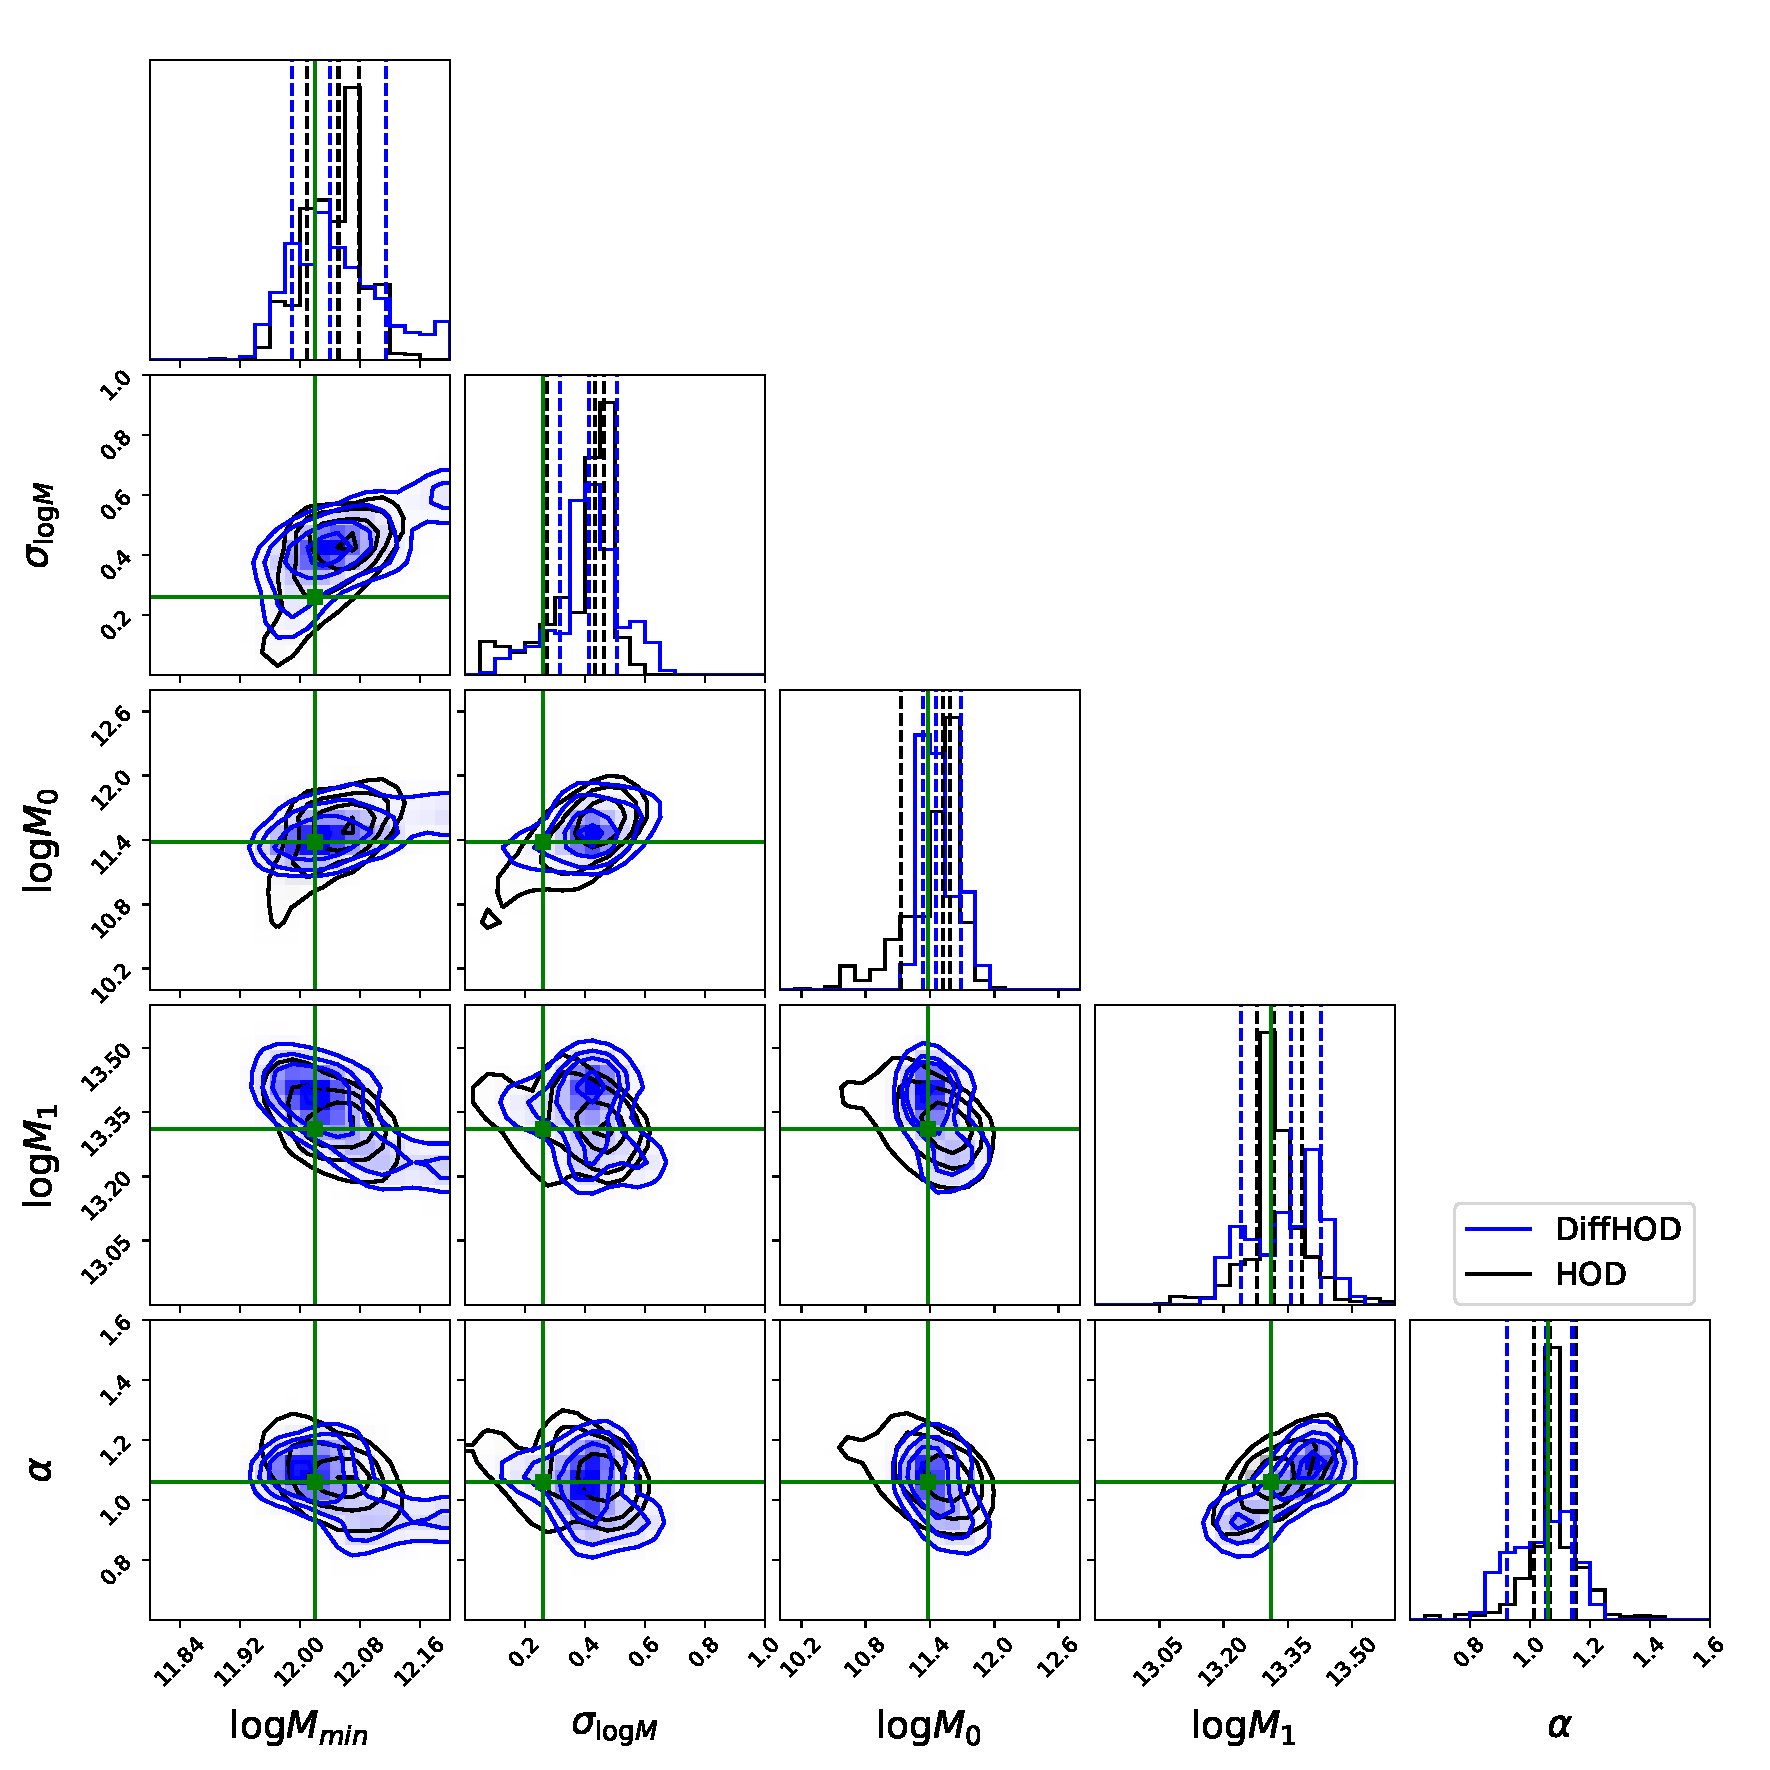
\includegraphics[width=0.50\textwidth]{paper/plots/HMC_MCMC_compar.pdf}
    \caption{Posterior distributions of the \cite{2007zheng} HOD parameters derived 
    using \dhod~with Hamiltonian Monte Carlo (red) and the standard HOD with Markov
    Chain Monte Carlo (black).
    We use a single mock galaxy catalog realization at the fiducial HOD parameter 
    values (green) as our observations. 
    We derive $20\times$ faster than standard HOD analyses with our \dhod~and HMC. 
    
    }
    %Output of the Hamiltonian Monte Carlo chain from the DiffHOD model (Red) and Markov Chain Monte Carlo chain from the HOD analysis (Black) for the mock dataset. }
    \label{fig:hmc}
\end{figure}


\section{Conclusions}
\label{sec:conclusion}
In this work we have constructed a differentiable stochastic HOD model going from a halo catalog to an observed galaxy power spectrum.
This allows us to use derivative-based optimization methods to quickly optimize for the underlying model parameters. 
This is the first time differentiable stochastic models have been used in the astrophysics literature. 
We find the \dhod~model provides a 
$20\times$ increase of speed versus the same analysis performed via MCMC with the standard HOD implementation.
\dhod~is an alternative to a number of recent works focusing on emulating galaxy clustering statistics \citep{2015ApJ...810...35K,2019MNRAS.484..989W,2020PhRvD.102f3504K,2020MNRAS.492.2872W}. 
Unlike emulator based methods, \dhod~works at the level of the halo catalog and allows fast, differentiable, generation of any summary statistic with respect to the HOD parameters.

In this work, we have focused on the \citet{2007zheng} HOD model, but this can be easily extended to a broad class of models. While standard HODs are based only on halo mass, in general various properties of the halos environment and formation history could effect the galaxy properties \citep{2006ApJ...639L...5Z,2007MNRAS.374.1303C}. Galaxy assembly bias has been argued \citep{2015MNRAS.446.1939F,2020MNRAS.493.5506H} to cause significant deviations between predictions of standard HOD models and those from hydrodynamical simulations. Decorated HOD models have been introduced to account for assembly bias \citep{2016MNRAS.460.2552H} and has been extended to include other possible effects \citep{2018MNRAS.478.2019Y}. These models still rely on stochastic discrete sampling for assigning centrals and satellites so they can be modelled in a differentiable way using the techniques described in this work.

\begin{table}
\centering
\def\arraystretch{1.5}
     \begin{tabular}{ c | c | c }
 \hline\hline  
     & \dhod & Standard HOD \\ \hline
    $\log(M_\textrm{min})$ & $12.05^{+0.03}_{-0.05}$ & $12.04^{+0.07}_{-0.05}$ 
\\
    $\sigma_{\log{M}}$ & $0.43^{+0.03}_{-0.16}$ & $0.41^{+0.09}_{-0.09}$
\\
    $\log M_0$ & $11.51^{+0.08}_{-0.38}$ & $11.36^{+0.23}_{-0.12}$ 
\\
    $\log{M_1}$ & $13.32^{+0.06}_{-0.05}$ & $13.36^{+0.07}_{-0.12}$
\\
 $\alpha$ & $1.07^{+0.08}_{-0.06}$ & $1.05^{+0.09}_{-0.13}$
\\
  \hline
 \end{tabular}
 \caption{Best fit values from the HOD analyses using the \dhod~and standard 
 HOD model. Uncertainties are estimate from the $16\%$ and $84\%$ quantiles.} 
 \label{table:values}
\end{table}
Differentiable HOD models have even more apparent applications in the case of dynamical forward model large scale reconstructions \citep{2017JCAP...12..009S} when paired with efficient differentiable halo finding methods \citep{2018JCAP...10..028M,2020arXiv201011847M,2019PhRvD.100d3515K}. While it is possible to perform these reconstructions by interpreting the galaxy field as a biased version of the dark matter field (i.e. in \cite{2021TARDISII}), inaccuracies in this prescription will result in biases that would be difficult to account for in cosmological constraints. Through joint inference of the HOD parameters with the initial density field, these astrophysical uncertainties can be rigorously marginalized out. Differentiable models are critical for this application as the optimization is highly multidimensional (approximately number of particles in the simulation) and would be computationally infeasible without gradient-based methods.

While in this work we have highlighted using our \dhod~model inside an HMC framework, one can take advantage of its automatic differentiation for a variety of first order optimization and parameter inference methods. For example standard Variational Inference relies on having well defined derivatives for the optimization of latent space parameters describing the likelihood surface \citep{peterson1987mean,2003PhDT.......250B,2016arXiv160100670B}. Variational inference could further accelerate parameter inference when compared to Hamiltonian Monte Carlo or nested sampling methods \cite{2018arXiv180306473G}.

\section*{Acknowledgements}
We thank Andrew Hearin and Matt Becker for very useful discussions and suggestions.
BH and CH are supported by the AI Accelerator program of the Schmidt Futures Foundation. 
SF is funded by the Physics Division of Lawrence Berkeley National Laboratory.
This research used resources of the National Energy Research Scientific Computing Center, a DOE Office of Science User Facility supported by the Office of Science of the U.S. Department of Energy under Contract No. DEC02-05CH11231.

%%%%%%%%%%%%%%%%%%%%%%%%%%%%%%%%%%%%%%%%%%%%%%%%%%

%%%%%%%%%%%%%%%%%%%% REFERENCES %%%%%%%%%%%%%%%%%%

% The best way to enter references is to use BibTeX:

\bibliographystyle{mnras}
%\bibliography{example} % if your bibtex file is called example.bib
\bibliography{ref}


%%%%%%%%%%%%%%%%%%%%%%%%%%%%%%%%%%%%%%%%%%%%%%%%%%

%%%%%%%%%%%%%%%%% APPENDICES %%%%%%%%%%%%%%%%%%%%%
\appendix
\section{Distributional Properties of \dhod\ Model}
\label{ap:1}
\begin{figure*}
    \centering
    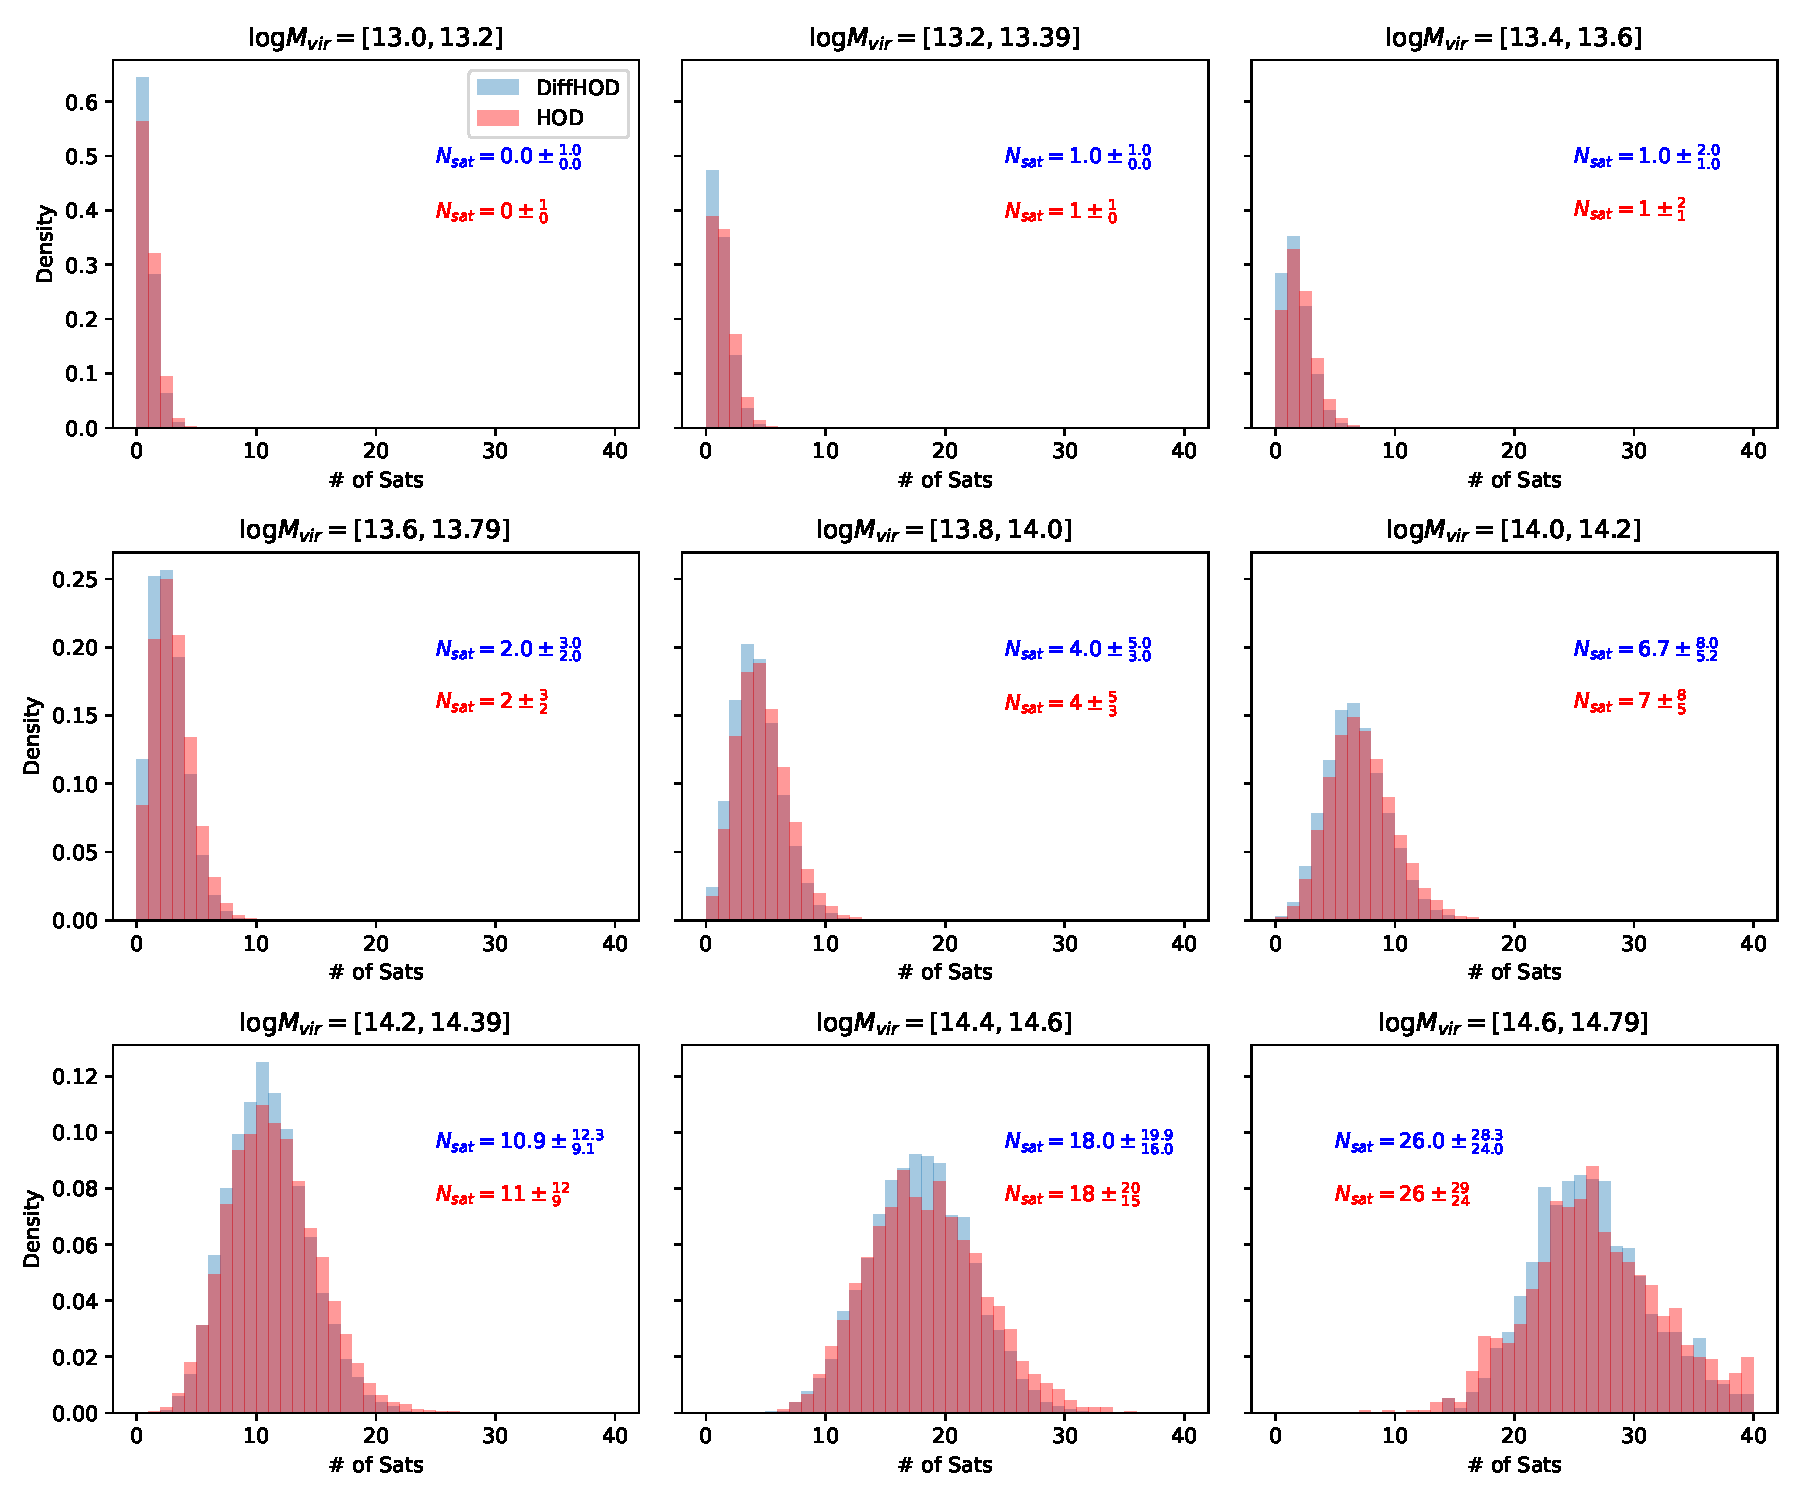
\includegraphics[width=0.90\textwidth]{paper/plots/distributions.pdf}
    \caption{Histogram showing the halo occupancy distribution from 100 independent samples from the complete halo catalog. We compare halos populated by our \dhod model as well as a standard HOD implementation. We show the median satellite occupation number, and quote error bars representing the 32\% and 68\% quartiles. We find excellent quantitative and qualitative agreement between the two distributions. }
    \label{fig:distribution}
\end{figure*}

In the main body of the work we sampled from a Bernouli Distribution rather than a pure Poisson Distribution due to the existing analytical tools to relax the Bernouli Distribution via the Gumbel-Softmax trick. This was demonstrated to be a valid approximation at the level of various summary statistics, such as halo occupancy distribution functions and resulting galaxy power spectrum. In this section we show the halo occupancy distribution as a function of halo mass.

We sample our satellite \dhod, at $\tau=0.02$, and the standard satellite HOD using the parameters in the main text 100 times in order to attain reasonable number statistics at the high mass bins. We show our results in \ref{fig:distribution}, finding quantitative good agreement between the models as calculated by their modal and variance properties. We calculate for each mass bin the 32\%, 50\% and 68\% percentiles. Since \dhod\ uses a relaxed distribution instead of sampling, it is possible to get non-integer number of satellites while for the standard HOD model all sampling is discretized. Qualitatively we see a slight skew near the peak of the distributions, however this does not appear to impact any of our resulting analysis 

%%%%%%%%%%%%%%%%%%%%%%%%%%%%%%%%%%%%%%%%%%%%%%%%%%


% Don't change these lines
\bsp	% typesetting comment
\label{lastpage}
\end{document}

% End of mnras_template.tex